%%% Local Variables:
%%% mode: latex
%%% TeX-master: "<none>"
%%% End:

\label{sec:joining}

After connecting with a splitter, incoming peers request (using a
reliable communication) to the splitter the current list of peers in
the team. To minimize the joining time, the peer sends a
$[\mathtt{hello}]$ message to each peer of the team, in parallel
with the reception of the list. When a peer of the team receives a
$[\mathtt{hello}]$, it adds the sender of the message to a table of peers
called $\text{forward}[]$. If a peer $P_i$ has an entry
$\text{forward}[P_j]=P_k$ then, each chunk received by $P_i$ and
originated at $P_j$ will be forwarded to $P_k$.

%), initializes
%the table $\mathrm{debt}[]$ (which stores the chunk debts between
%neighbor peers), and (3) sets the variable $\mathrm{neighbor}$ with an
%index to $\mathrm{forward}[]$ (see
%Sec.~\ref{sec:chunk_DBS_processing}).

The splitter, in a loop: (1) listens to the incoming peers, (2) sends
the list of peers in the team, and (3) adds the incoming peer to the
list.

\begin{comment}
\begin{figure*}
  %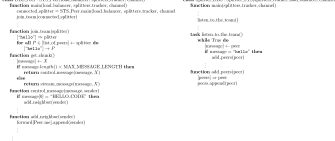
\includegraphics[width=\textwidth]{joining}
  \fig{1000}{10cm}{joining} \caption{Code related to team
    joining.\label{fig:joining}}
\end{figure*}

The new pseudo-code related to joining a team is describen in the
Fig.~\ref{fig:joining}.
\end{comment}
